\chapter{Discussion}
\label{chap:discussion}

\section{Development decisions}
\subsection{Using scriptable objects}
\label{sec:scriptableObjects}
When we first started working on the modifier architecture for Dockit League, we had to find an easy to use and extendable way of creating new modifiers. Having recently seen a talk from \emph{Unity Europe 2016}~\cite{scriptableObjectsTalk} about how scriptable objects can be used for these types of use cases, we decided to base the architecture around them. Using scriptable objects instead of \emph{MonoBehaviour} has a wide range of advantages:
\begin{itemize}
    \item A scriptable object is not reset when exiting play mode compared to a \emph{MonoBehaviour} object. This means that any values tweaked in the inspector while playing stay saved.
    \item Scriptable objects can be referenced instead of copied when instantiated, helping decrease unwanted redundancy for complex objects. 
    \item A scriptable object can be referenced from any scene while keeping cross-scene references of \emph{MonoBehaviour} objects can be tricky. 
    \item Scriptable objects provide better version control granularity as one file gives one object without anything additional like transform components. 
\end{itemize}

Scriptable objects also have some disadvantages:
\begin{itemize}
    \item Scriptable objects have very few callbacks compared to a \emph{MonoBehaviour} object. \emph{OnEnable()}, \emph{OnDisable()} and \emph{OnDestroy()} are the only ones. This can be worked around by having a proxy \emph{MonoBehaviour} that calls functions within the scriptable object. 
    \item Scriptable objects contain shared data. This means that any object references during runtime only should be acquired and used in method scope. 
\end{itemize}

In the case of our project. Using scriptable objects for modifiers and shop items gives us the ability to create and quickly edit data directly in the editor as well as being able to attach some additional code if necessary. 
In the case of modifiers, using scriptable objects makes it very easy to define custom behaviour through the use of the multiple callbacks that exist within the base \emph{Modifier} class. These can be overridden to perform code for the server only, on all clients and locally which gives us the amount of control we want when working on a networked multiplayer game. 
In the case of shop items, using scriptable objects provides a reusable interface that allows us to quickly add items without having to worry about editing other dependent components as the shop itself handles instantiation and placement of these.  

A more technical look at how scriptable objects are used for modifiers and shop items can be found in Section~\ref{sec:modifiers} and Section~\ref{sec:scriptableObjectsShop}.
    
\subsection{Moving from Confluence to ShareLaTeX for writing the thesis}
As seen in Appendix~\ref{app:projectPlan} we had originally planned to use Confluence as the thesis container as that would mean having a centralized hub for documentation and the thesis. We eventually started moving away from Confluence and ended up only using it to document any Scrum related meetings and started using ShareLaTeX instead. The reason for this is that it allows the thesis to look more professional due to the template style sheet as well as providing a lot of utility tools that make writing the thesis easier. Some of these include easy access to PDF compilation, BibTeX for formatting and automating references as well as being able to work on the thesis in a parallel manner similar to Google Docs. Another benefit of using ShareLaTeX is that less time is spent worrying about text formatting as this is mostly handled by the stylesheet from the thesis template. 

\subsection{Decreasing the amount virtual functions using interfaces}
The \emph{Ability} base class in an important intermediary component for making the docking kits work with networked code. The script itself is not a \emph{NetworkBehaviour} so it instead employs virtual functions that get called by networked components to provide synchronized behaviour. One of the issues we experienced throughout development was the fact that this class would get exceedingly bloated with virtual functions as more features were required. The worst offender were the functions that allowed abilities to have server callbacks, providing similar functionality to the \emph{ClientRpc} attributes of \emph{NetworkBehaviour}'s. The issue here was that whenever we wanted to pass parameters we had to first create a new command in the \emph{Docking} script due to not being able to overload commands or provide generic parameters. We then had to create a corresponding virtual function taking the parameters in the \emph{Ability} class. 

We ended up using interfaces to somewhat alleviate the code bloat. The difference with using interfaces is that we no longer need to create the additional virtual functions in \emph{Ability} for each new type of parameter. Instead, individual abilities can implement the \emph{IServerCallback} interface which supports generic parameters. Using this approach decreases the code bloat a little bit, but we still need to create new commands in \emph{Docking} due to the inherent limitations of commands. In any case it helps reduce a little bit of code bloat so we found it a worthwhile solution. 

\subsection{Providing ergonomic controls when using a twin stick scheme}
\label{sec:ergonomicControls}
During the early design phase one of the things we had to decide on was how many abilities each docking kit would have. We wanted each kit to have enough depth so that players would have to spend some time properly learning each kit and improving their play through experience, but we also had to take into account the control scheme that we were targeting. The abilities of each kit should be easy to access when using a controller while moving about and aiming at the same time. This leaves us with a rather limited selections of buttons to use. 

We have the shoulder buttons, triggers and stick buttons available. We decided that each kit would have four abilities each as the triggers and shoulder buttons are the most ergonomic to use with the dual stick scheme. Using the stick buttons for additional abilities would also have been possible, but we could imagine some imprecise aiming if for example an ability was bound to the right stick button. Less frequently used functionality like opening the shop and docking/undocking could then mapped to the primary ABXY, Start and Select buttons.

\subsection{Updating game engine versions during development}
\label{sec:updatingGameEngine}
Whenever developing games in a constantly updated engine like Unity or Unreal it is inevitable that new versions are released. These new versions come in different shapes and forms. Minor releases mostly contain bug fixes and small changes while major releases introduce new functionality and might end up deprecating old features. In cases where changes or new functionality might be beneficial for the project, one has to see whether spending the time and resources on the upgrade is worth it. 

While testing the game during sprint reviews, one of the issues we ended up experiencing at times were random disconnects with seemingly limited error messaging given for debugging. Researching into the issue a bit on the Unity forums suggested it could be related to the 4KB/s bandwidth limit of Unity. At the same time the issue could simply be related to a inconsistent wireless network at the location we were testing, but we started to think a bit about bandwidth optimization anyways. 

One of the most apparent optimization's we could perform was to move from Unity3D back to Unity2D with the release of Unity 5.6. We originally started working with Unity3D due to the fact that it provided \emph{NavMeshes}~\cite{unityNavMeshes} which would be beneficial in the case that we had the time to work on player bots. Unity 5.6 introduced \emph{NavMeshes} for the (x, y) plane making it possible for us to port the game back to 2D. Doing so would substantially decrease network bandwidth usage since there were no dependencies on 3D components. 

One of the pieces of data we synchronise often are \emph{Vector3}'s consisting of three floating point values. Synchronized \emph{Rigidbody} components in particular consist of many physics related vectors~\cite{unityRigidbody}. Moving to Unity2D would cut the bandwidth usage for any Rigidbody and vector synchronization by $\frac{1}{3}$ which is a fairly significant improvement in network performance. Another side effect of moving over to 2D would be cheaper ray casting. The \emph{FieldOfView} component uses a lot of ray casts to create its view mesh so the performance of this script in particular would improve. 2D Raycasts also give some additional quality of life functionality like providing sorted arrays in order of distance from the origin point when raycasting for multiple colliders.  

Another useful piece of functionality that only works with Unity2D is the \emph{PolygonCollider2D} component which allows Unity to dynamically create colliders out of sprites. Unity offers similar functionality for 3D using the \emph{MeshCollider} component, but creating sprites is generally far quicker and easier than using 3D models for simple shapes like cones and hollow circles. 

We ultimately decided against transferring over to Unity2D due to the fact that the release of Unity 5.6 happened very late into the development cycle. We thought that moving over to Unity2D would take too much time and given that we had no conclusive evidence of hitting the bandwidth limit we would rather spend the resources on writing and improving the thesis instead.  

\subsection{Player field of view versus raycasts for visibility checking}
One idea that we thought of while developing was to use the field of view component for visibility checking rather than regular ray casting. This would allow abilities like the flash grenade in the brawler kit to only stun players who had the grenade in their field of view at the time of explosion rather than using a raycast + dot product. We ultimately decided against implementing this due to a few reasons. 

The first reason is that the field of view is fairly computationally expensive. The component uses many raycasts to dynamically generate a mesh that we use as a visibility mask for the players. It would not be possible to directly synchronise the generated meshes so we would have to synchronise the various variables for the component itself and reconstruct the field of view on the server. Doing so would allow us to have a player local field of view for the sake of responsiveness while using the server's version for any visibility checking. This could work if the server was ran as a dedicated server, but our project is primarily focused on trying to create a MOBA using peer to peer connectivity so a implementation like this would not be very effective as it would place a lot of extra load on the host player. 

A server authoritative visibility check like this would be far better for security reasons compared to local checking. We currently have a middle ground where the server uses raycasts and dot products to check player face directions. This is independent of the field of view component so we have less control in regards to limiting the view angles as the server would need to acquire the view angle of the clients to check consistently with their current field of view.

Another issue is that keeping the field of view synchronized would take a fair share of additional bandwidth if we want the server to keep itself updated frequently. Given the fact that players move and are able to rotate quickly and arbitrarily, a very high update rate or interpolation would have to be employed for the server to stay consistent with the local player. Since players can rotate arbitrarily and quickly, using interpolation for the field of view would be somewhat of a challenge as determining whether the player rotated clockwise or counter clockwise to the current rotation would be hard without synchronising additional data. This would require a fairly massive rework of the current implementation.  

\subsection{Sticking with dual stick controls}
Dockit League is primarily developed with a twin stick controller setup in mind. This is mostly due to the fact that other control options were outside of the scope for the project. One might think that providing similar controls through the use of a mouse would be simple, but it brings somewhat of a balancing issue. 
Making the player face towards the direction of the mouse pointer is generally what we would think of as the simplest and most intuitive implementation of the mouse control scheme. The main problem with this implementation is that aiming becomes easier for players using a mouse. To give an example, two players standing still at different positions want to fire at each other with a projectile. One uses a mouse while the other uses a controller. The player using the mouse can simply hover the mouse cursor over the other player for accurate aim while the player using the controller needs to aim by approximately pointing the right stick in the correct direction.  

To provide similar behaviour between the controller and mouse options we would need to make the mouse controls work more similarly to that of a controller stick. The mouse cursor could be hidden and reset to the center of the screen each frame while recording any changes in mouse movement as a direction vector. This vector could then be used to make the player point in the same direction that the mouse is moving. This would balance the two control schemes to some degree, but we believe that mouse controls like the ones we described might end up feeling too unintuitive for players. Due to this we ended up deciding to stick with the controller dual stick scheme for our project scope. 
    
\section{Experiences with the HLAPI of Unity}
The HLAPI of Unity has been very useful for us when developing \emph{Dockit League}. It provides a good high level API that has somewhat of a learning curve, but is generally easy to use once we had worked more with it. It is not without its flaws however. Certain functionality like host migration is still broken to this date as noted by other developers on the Unity forums~\cite{forumsUnityNetworkFeedback} and Reddit~\cite{redditUnityNetwork}. Host migration in particular is a very essential feature for a peer to peer based game as it prevents everyone from disconnecting when the host disconnects. There is also somewhat lacking debugging tools available for the networking. A lot of error messages related to disconnects are vague and it is also not possible to directly measure bandwidth usage in the profiler. This would be useful for developers wanting to know how much of the bandwidth limit they used so they could optimize parts of the networking accordingly. 

The base documentation for Unity's network components is fairly decent in our opinion, but there are parts where the quality of documentation drops to an unacceptable level. The \emph{LobbyManager} and its lobby related systems are horribly documented with only two example projects available in the Asset Store. There is a distinct lack of overarching documentation for how the lobby components work in these projects. To quote the documentation from one of the sample projects on the Asset Store~\cite{unityAssetLobby}: 

\begin{quote}
"The main prefab is in "Prefabs/LobbyManager". This is a canvas with the LobbyManager script on it.
It have multiple child that setup the UI \& different "screens" of the lobby (i.e. Server List, Player Lsit etc...)

Everything above the "Unity UI Lobby" section in the Manager Inspector is from UnityEngine.Networking.NetworkLobbyManager, so see the doc
for it to see an explaination for all of them.

Prematch countdown is the time between all players being ready \& the game starting.

The Lobbymanager script have reference to all the different screens for easy access.
*if you totally replace one of those screens, set its reference there*"
\end{quote}

The documentation in the project is filled with badly written grammar and refers to documentation that barely exists on Unity's web pages. 

\section{Observations from sprint statistics}
\begin{figure}[tbph]
    \centering
    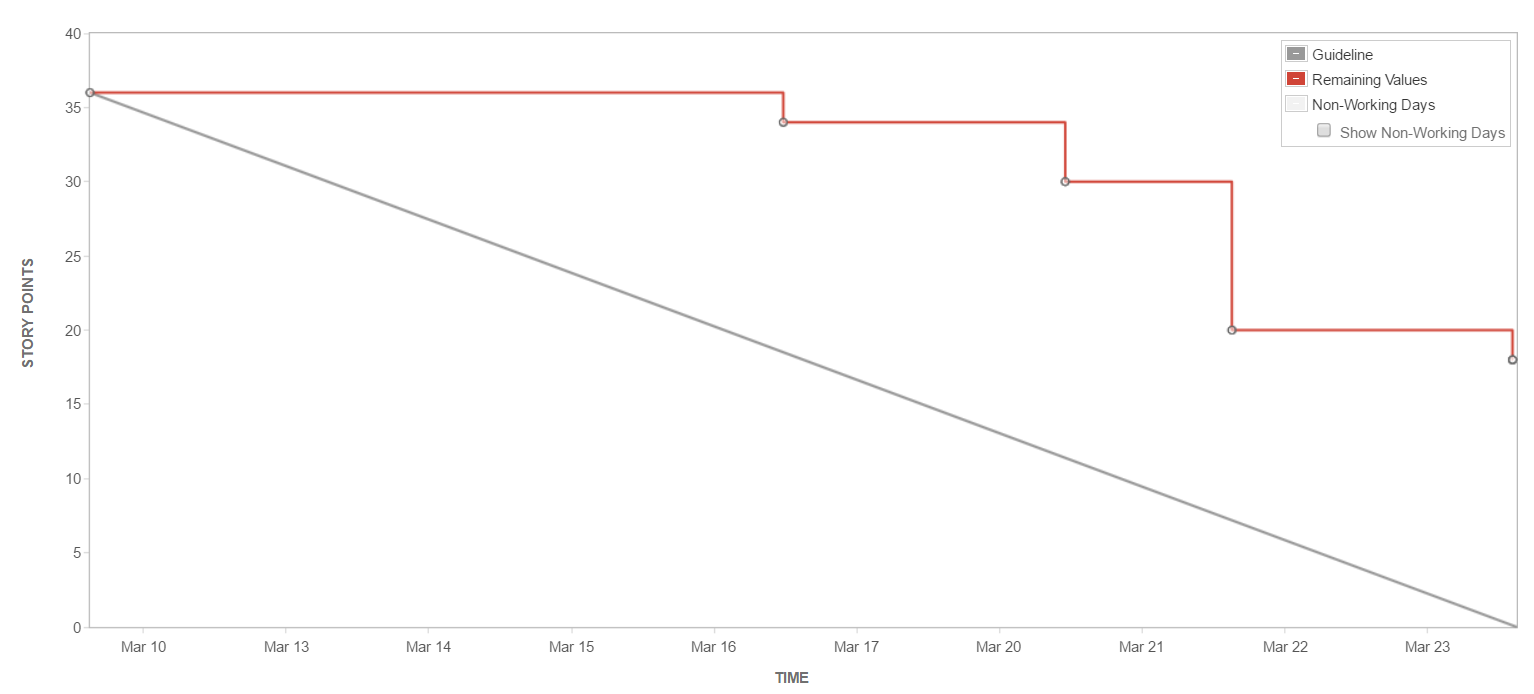
\includegraphics[width=\textwidth]{images/DOCKLSprint4}
    \caption[Burndown chart from the 4th sprint]{The burndown chart for the 4th sprint shows how sprints generally progressed on average throughout the project.}
    \label{fig:burndownChart}
\end{figure}

We will take a brief look at Figure~\ref{fig:burndownChart} which illustrates the burndown chart of the 4th sprint during development as it shows data that was fairly consistent throughout the other sprints. 

The first observation is that most issues generally were finished throughout the second week of the sprint rather than issues regularly finished as the guideline suggests. This is mostly due to the fact that the issues were rather large and not split up into subtasks very often. Doing so would better reflect project progress on Jira, but at the same time this would incur a fair amount of additional overhead per sprint by having to set up subtasks per issue. 

The next apparent observation is overscope. Most of the sprints after sprint 1 ended up having some overscope. The overscope was mostly related to being able to finish a docking kit while also working on other functionality of the game at the same time. This could certainly have been improved by looking at the statistics of previous sprints and manage expectations accordingly. The estimations for some of the game functionalities ended up being estimated for lower story point values than they required due to unexpected issues and bugs which resulted in a lack of resources needed to finish some of the docking kits for the sprint. 

\subsection{Looking at the use of Scrum in retrospect}
In relation to actually working on docking kits, fortnightly sprints ended up fitting well. Designing and implementing the base functionality of most kits required one week of time while the other week was spent on bug fixing and polish. 

Working with Jira allowed us to setup sprints and issues in a tidy manner, but had a lot of additional functionality we never used although we can imagine a lot of it being useful for managing larger teams. 

Despite there having been some overscope during development, using Scrum allowed us to continue developing new increments without necessarily cutting or rushing core functionality of the game due to direct deadlines. The benefit of also having a rather relaxed scope for the game was that it meshed well with Scrum and agile development in general. 

The daily standup meetings in particular were quite useful to us. They helped each group member to stay updated with the different components of the project and worked well as a daily discussion around core functionality requirements as the development progressed. There was a fair amount of uncertainty around the requirements for the core components at the start of the development process. As more kits were implemented we started being able to use these daily meetings to discuss the various requirements our components needed to work with the designs of the different docking kits. 